\documentclass[border=10pt]{standalone}
\usepackage[T1]{fontenc}
\usepackage{amsmath,amsfonts}
\usepackage{tikz}
\usetikzlibrary{shapes.geometric} % Cylinder
\usetikzlibrary{shadows.blur,arrows.meta,bending,positioning}
\usetikzlibrary{%
	calc,%
	decorations.pathmorphing,%
	fadings,%
	shadings%
}

\pgfdeclaredecoration{lightning bolt}{draw}{
\state{draw}[width=\pgfdecoratedpathlength]{
  \pgfpathmoveto{\pgfpointorigin}%
  \pgfpathlineto{\pgfpoint{\pgfdecoratedpathlength*0.6}%
    {-\pgfdecoratedpathlength*.1}}%
  \pgfpathlineto{\pgfpoint{\pgfdecoratedpathlength*0.55}{0pt}}%
  \pgfpathlineto{\pgfpoint{\pgfdecoratedpathlength}{0pt}}%
  \pgfpathlineto{\pgfpoint{\pgfdecoratedpathlength*0.4}%
    {\pgfdecoratedpathlength*.1}}%
  \pgfpathlineto{\pgfpoint{\pgfdecoratedpathlength*0.45}{0pt}}%
  \pgfpathclose%
}%
}
\begin{document}
  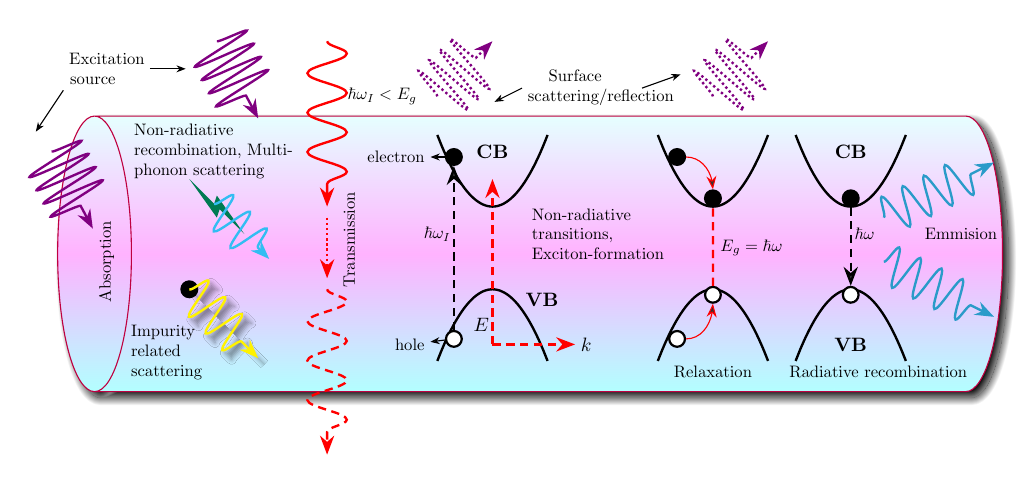
\begin{tikzpicture}[
    withShadow/.style={
      cylinder, 
      minimum height=12cm, 
      minimum width=3.5cm,     
      aspect=4,
      %cylinder end fill=purple!10!magenta, 
      draw=purple,
      blur shadow={
        shadow blur steps=30,
        shadow blur radius=1mm,
        shadow opacity=100,shadow blur steps=100,
        color=purple,
        fill=purple,
      }
    },
  ]
  \node[withShadow,
  left color=cyan!10,
  right color=cyan!30,
   middle color=magenta!30,
   rotate=-180,
      shading angle=0,](c2)at(5,-2){};

\begin{scope}[scale=0.7]


% transimission
\node[scale=0.6] at (4,0.){$\hbar\omega_{I}<E_{g}$};
\draw[decoration={snake,amplitude=2.5mm,segment length=5mm,post length=2mm},decorate,red,-{Stealth},line width=.3mm] (3,1) -- ++(0,-3);
\draw[-{Stealth},densely dotted, line width=0.3mm,red] (3,-2.2)--++(0,-1.1);
\draw[decoration={snake,amplitude=2.5mm,segment length=5mm,post length=2mm},decorate,red,-{Stealth},line width=.3mm,densely dashed] (3,-3.5) -- ++(0,-3);
\node[rotate=90,scale=0.6] at (3.4,-2.6){Transmission};
\draw[decoration={snake,amplitude=4mm,segment length=1.9mm,post length=3mm},decorate,violet,-{Stealth},line width=.3mm] (1,1) -- ++(0.75,-1.4);


% excitatio source
\draw[decoration={snake,amplitude=4mm,segment length=1.9mm,post length=3mm},decorate,violet,-{Stealth},line width=.3mm] (-2,-1) -- ++(0.75,-1.4);
\node[scale=0.6,text width=1cm, align=center](es) at (-1.25,0.5) {Excitation source};
\draw[-{Stealth[scale=0.7]}] ([xshift=0.5cm]es.east)--([xshift=1.15cm]es.east);
\draw[-{Stealth[scale=0.7]}] ([xshift=0.cm]es.south west)--([xshift=-0.5cm,yshift=-0.75cm]es.south west);

% non-radiative
\node[text width=3.5cm,scale=0.6] at (1,-1) {Non-radiative\\ recombination, Multiphonon scattering};
\fill [green!60!blue!80!black, decoration=lightning bolt, decorate] 
(0.5,-1.5) -- ++ (1,-1);
\draw[decoration={snake,amplitude=2.5mm,segment length=3mm,post length=2mm},decorate,cyan!80,-{Stealth},line width=.3mm] (0.95,-1.95) -- ++(1,-1);

%yellow arro impurity
\node[solid,circle,inner sep=0pt,minimum size=2mm,fill=black,thick,draw] (e2) at (0.5,-3.5){};
\draw[decoration={snake,amplitude=2.5mm,segment length=3mm,post length=2mm},decorate,yellow,-{Stealth},line width=.3mm,blur shadow={shadow blur extra rounding}] (0.5,-3.5) -- ++(1.25,-1.25);
\node[text width=2cm,scale=0.6] at (0.3,-4.65) {Impurity related \\scattering};


%purple arrows excitation source
\node[rotate=90,scale=0.6] at (-1,-3) {Absorption};
\draw[decoration={snake,amplitude=4mm,segment length=1.9mm,post length=3mm},decorate,violet,-{Stealth},line width=.3mm,densely dotted] (5,0) -- ++(1,1);
\draw[decoration={snake,amplitude=4mm,segment length=1.9mm,post length=3mm},decorate,violet,-{Stealth},line width=.3mm,densely dotted] (10,0) -- ++(1,1);


% dashed purple scattering surface
\node[text width=2cm,scale=0.6,align=center](sf) at (7.5,0.15) {Surface\\ scattering/reflection};
\draw[-{Stealth[scale=0.7]}] (sf.west)--([xshift=-0.5cm,yshift=-0.25cm]sf.west);
\draw[-{Stealth[scale=0.7]}] ([xshift=0.25cm]sf.east)--([xshift=0.95cm,yshift=0.25cm]sf.east);


%incide non-radiative
\node[text width=3cm,align=left,scale=0.6] at (8,-2.5) {Non-radiative\\ transitions,\\Exciton-formation};

% first bands
\draw[ line width = 0.3mm,xshift=6cm,yshift=-2cm]   plot[smooth,domain=-1:1] (\x, {1.3*\x*\x});
\draw[ line width = 0.3mm,xshift=6cm,yshift=-2cm]   plot[smooth,domain=-1:1] (\x, {-1.3*\x*\x-1.5});
\draw[-{Stealth},densely dashed,red, line width=0.3mm] (6,-4.5)--(6,-1.5);
\draw[-{Stealth},densely dashed,red, line width=0.3mm] (6,-4.5)--(7.5,-4.5);
\node[scale=0.7] at(7.7,-4.5){$k$};
\node[scale=0.7] at(5.8,-4.15){$E$};
\node[scale=0.7] at (6,-1){$\mathbf{CB}$};
\node[scale=0.7] at (6.9,-3.7){$\mathbf{VB}$};
\node[solid,circle,inner sep=0pt,minimum size=2mm,fill=white,thick,draw] (h) at (5.3,-4.4){};
\node[solid,circle,inner sep=0pt,minimum size=2mm,fill=black,thick,draw] (e) at (5.3,-1.1){};
\draw[-{Stealth},densely dashed, line width=0.3mm] (h)--(e);

\node[scale=0.6](t1) at (4.25,-1.1){electron};
\draw[-{Stealth[scale=0.7]},inner sep=0mm] (e)--(t1);
\node[scale=0.6] at (5,-2.5){$\hbar\omega_{I}$};
\node[scale=0.6](t2) at (4.5,-4.5){hole};
\draw[-{Stealth[scale=0.7]},inner sep=0mm] (h)--(t2);

%second and third bands
        \draw[ line width = 0.3mm,xshift=10cm,yshift=-2cm]   plot[smooth,domain=-1:1] (\x, {1.3*\x*\x});
        \draw[ line width = 0.3mm,xshift=10cm,yshift=-2cm]   plot[smooth,domain=-1:1] (\x, {-1.3*\x*\x-1.5});
        \node[solid,circle,inner sep=0pt,minimum size=2mm,fill=white,thick,draw] (h2) at (10,-3.6){};
        \node[solid,circle,inner sep=0pt,minimum size=2mm,fill=black,thick,draw] (e2) at (10,-1.85){};
        \draw[red,densely dashed, line width=0.3mm] (h2)--(e2);
        \node[solid,circle,inner sep=0pt,minimum size=2mm,fill=white,thick,draw] (h3) at (9.35,-4.4){};
        \node[solid,circle,inner sep=0pt,minimum size=2mm,fill=black,thick,draw] (e3) at (9.35,-1.1){};
        
        \path[-{Stealth},red] (h3) edge [out=0, in=270] node {} (h2);
        \path[-{Stealth},red] (e3) edge [out=0,in=90] node {} (e2);

        \node[scale=0.6] at (10.7,-2.75){$E_{g}=\hbar\omega$};

        \draw[ line width = 0.3mm,xshift=12.5cm,yshift=-2cm]   plot[smooth,domain=-1:1] (\x, {1.3*\x*\x});
        \draw[ line width = 0.3mm,xshift=12.5cm,yshift=-2cm]   plot[smooth,domain=-1:1] (\x, {-1.3*\x*\x-1.5});
        \node[solid,circle,inner sep=0pt,minimum size=2mm,fill=white,thick,draw] (h4) at (12.5,-3.6){};
        \node[solid,circle,inner sep=0pt,minimum size=2mm,fill=black,thick,draw] (e4) at (12.5,-1.85){};
        \draw[-{Stealth},densely dashed, line width=0.3mm] (e4)--(h4);  
        \node[scale=0.7] at (12.5,-1){$\mathbf{CB}$};
        \node[scale=0.7] at (12.5,-4.5){$\mathbf{VB}$};
        
        \draw[decoration={snake,amplitude=2.5mm,segment length=3mm,post length=2mm},decorate,cyan!80!black,-{Stealth},line width=.3mm] (13.1,-2.2) -- ++(2,1);

        \node[scale=0.6] at (14.5,-2.5){Emmision};
        \node[scale=0.6] at (12.75,-2.5){$\hbar\omega$};

        \draw[decoration={snake,amplitude=2.5mm,segment length=3mm,post length=2mm},decorate,cyan!80!black,-{Stealth},line width=.3mm] (13.1,-3) -- ++(2,-1);
        
        \node[scale=0.6,anchor=center] at (10,-5){Relaxation};
        \node[scale=0.6,anchor=center] at (13,-5){Radiative recombination};
      \end{scope}
  


  \end{tikzpicture}
\end{document}